%!TEX root = ../report.tex
\chapter{Methodology}

\section{Semantic segmentation architectures}
Inline with the goal of the project to use resource efficient deep learning in terms of inference time and storage memory, the deepLab v3+ model with mobileNetv2 and xception variant was chosen. In order to better understand deepLabv3+, we consider breaking down the architectures of the previous versions of deepLab leading upto the current version. The different versions of deepLab are deepLab, deepLabv2, deepLabv3 and deepLabv3+ (the current version also called as deepLabv4).

\subsection{DeepLab}

Fully Convolutional networks were introduced by [] for the task of semantic segmentation. The predictions obtained with the help of this network were coarse and the object boundaries were not sufficiently delineated. In order to overcome these difficulties, the authors of deepLab proposed the use of atrous convolutions and fully-connected Conditional Random Fields (CRF).

Atrous convolutions, also called as dilated convolutions, is be used to gather a better global context with enlarged field-of-view on the feature maps. A atrous rate called r, determines the field-of-view of an atrous convolution. With increase in dilation rate, a greater region in the feature map is convolved over. This leads to gathering of more global context. However, it is worth noting that there is no increase in the number of parameters in the convolution filter. Only the convolved region in the input feature map changes. When the dilation rate is 1, usual convolution is performed. The figure \ref{Fig:atconv} illustrates atrous convolution. 

	\begin{figure}[!htb]
		\begin{subfigure}{.3\textwidth}
			\centering
			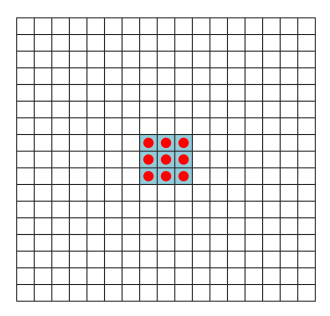
\includegraphics[width=1.03\linewidth]{images/r_1}
			\caption{Atrous rate = 1}
		\end{subfigure}
		\begin{subfigure}{.3\textwidth}
			\centering
			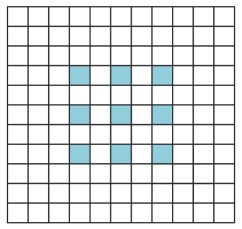
\includegraphics[width=1\linewidth]{images/r_2}
			\caption{Atrous rate = 2}
		\end{subfigure}
		\begin{subfigure}{.3\textwidth}
			\centering
			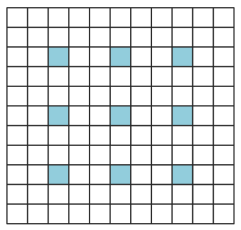
\includegraphics[width=1\linewidth]{images/r_3}
			\caption{Atrous rate = 3}
		\end{subfigure}
		\caption{Illustration of atrous convolution with three different atrous rates.}
		\label{Fig:atconv}
	\end{figure}
	
Fully-connected Conditional Random Fields (CRF), is used to post process the prediction of the CNN to improve object delineation. Every pixel in the output feature map is connected to every other pixel resulting in pairwise terms. In each pairwise term, based on color and position, the similarity between pixels is determined and a class is assigned for the pixels.


\subsection{DeepLabv2}

Source: http://www.davidtvs.com/exploring-semantic-segmentation-dnn/
In DeepLabv2, Atrous Spatial Pyramid Pooling (ASPP) was used in addition to the existing architecture. The authors also use deeper ResNet network to imrpove accuracy.

Atrous Spatial Pyramid Pooling, is used to create multiscale feature representations. Atrous convolutions with different atrous rates are applied to the same feature map. The resulting feature maps from each atrous convolution is processed in seperate branches in a similar fashion as in deepLabv1 by using two 1$\times$1 convolutions. Each of the branches are then fused together to obtain multiscale information. The difference between in architecture between deepLabv1 and deepLabv2 is illustrated in \ref{Fig:v1vsv2}.

	\begin{figure}[!htb]
		\centering
		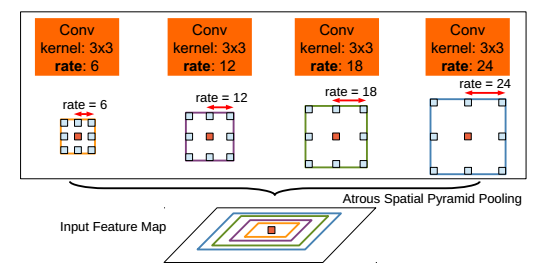
\includegraphics[width=0.6\linewidth]{images/aspp}
		\caption{Illustration of Atrous Spatial Pyramid Pooling (ASPP). Atrous convolutions with 4 different rates convolve on the same input feature map. The field-of-view of each atrous rate is shown using different colors.}
		\label{Fig:aspp}
	\end{figure}
	
	\begin{figure}[!htb]
		\begin{subfigure}{.5\textwidth}
			\centering
			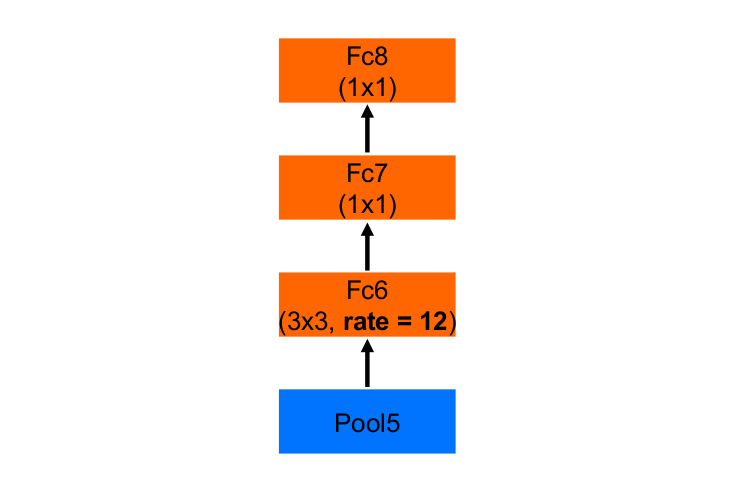
\includegraphics[width=1.03\linewidth]{images/v1_largeFOV}
			\caption{Large field-of-view in DeepLabv1}
		\end{subfigure}
		\begin{subfigure}{.5\textwidth}
			\centering
			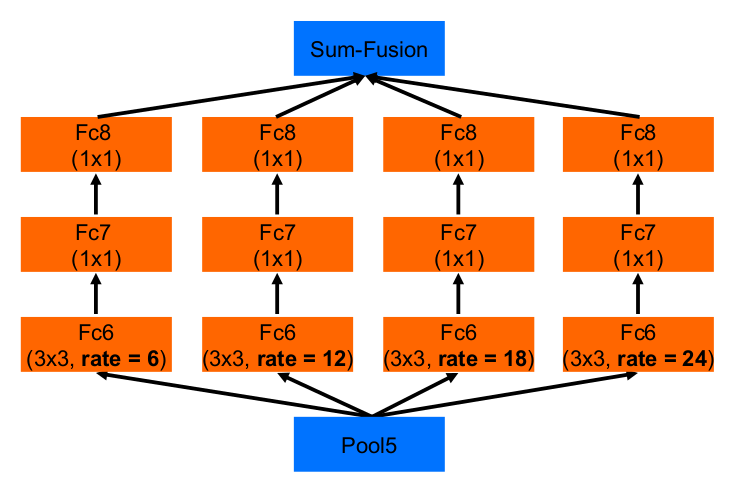
\includegraphics[width=1\linewidth]{images/v2_aspp}
			\caption{ASPP in DeepLabv2}
		\end{subfigure}
		\caption{Illustration of the difference in architecture between DeepLabv1 and DeepLabv2.}
		\label{Fig:v1vsv2}
	\end{figure}
	
\subsection{DeepLabv3}
In this version of deepLab, the contributions include improvements to the context module, the use of batch normalization and multi-grid method.

The authors experiment with two different modules to handle context one being a cascade module and the other being an improved version of ASPP module. The cascade module is formed by repeating the last block from ResNet and replacing convolutions with atrous convolutions. The authors report that performing this repetition upto three times improves performance. 	The cascade module is illustrated in \ref{Fig:contextmodulea}. The ASPP module used in deepLabv3 is similar to the one used in deepLabv2. However, there are a few changes including

	\begin{figure}[!htb]
		\begin{subfigure}{1\textwidth}
			\centering
			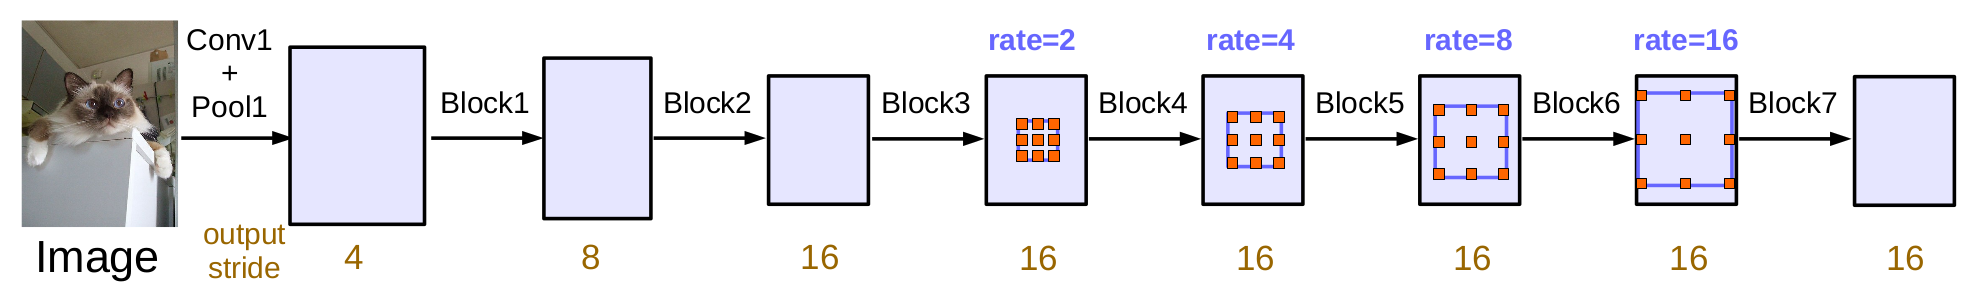
\includegraphics[width=1\linewidth]{images/cascade_module}
			\label{Fig:contextmodulea}
			\caption{cascade module in DeepLabv3}
		\end{subfigure}
		\begin{subfigure}{1\textwidth}
			\centering
			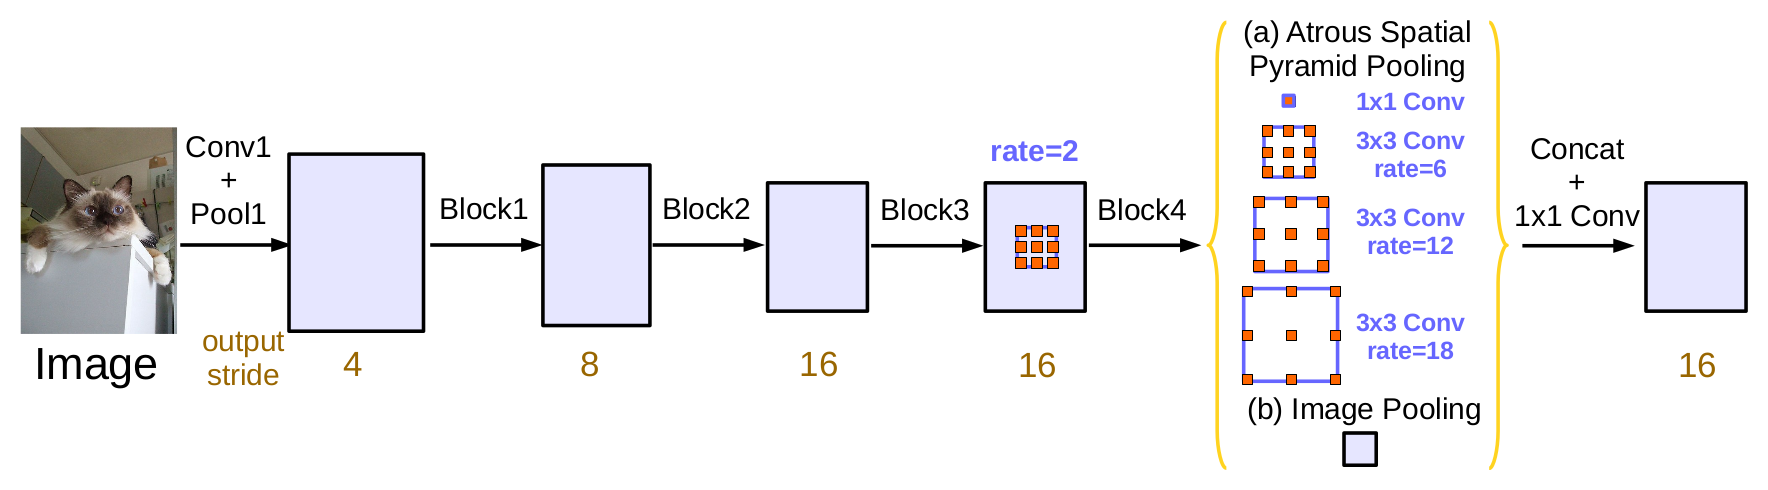
\includegraphics[width=1\linewidth]{images/aspp_module}
			\label{Fig:contextmoduleb}
			\caption{ASPP module in DeepLabv3}
		\end{subfigure}
		\caption{Illustration of two different context modules used in deepLabv3.}
		\label{Fig:contextmodule}
	\end{figure}

Batch Normalization is applied to every layer in the context module. This change leads to improvement in the Mean IOU attained in PASCAL VOC 2012 dataset. 

Multi-grid method is employed to 

\subsection{DeepLabv3+}

DeepLabv3+ is designed to combine the ability of ASPP module which can capture rich context information and the ability of encoder-decoder networks which can produce sharp object boundary delineation. 

\subsection{MobileNetv2}

% to cite: https://towardsdatascience.com/mobilenetv2-inverted-residuals-and-linear-bottlenecks-8a4362f4ffd5

% mobileNetv2 building block: https://ai.googleblog.com/2018/04/mobilenetv2-next-generation-of-on.html 

The mobileNetv2 architecture is designed to work on mobile and embedded devices where computational resources are limited. The authors state that their main contribution is the use of a novel layer module called the inverted residual with linear bottleneck. 

Depthwise separable convolutions, known for its efficiency, is used in this work. Standard convolution layers are replaced with two layers where the first layer performs depthwise convolution and the second layer performs pointwise convolution. A depthwise convolution layer uses a single fiter per input channel to perform convolution. The pointwise convolution layer consists of 1$\times$1 convolutions which perform weighted linear combination on the input channels and project them to a new channel space. This factorization of standard convolution layer into two separate depthwise and pointwise layers leads to roughly $k^2$ times reduction in computation cost where k is the kernel size of the convolutional filter. 

In the original residual block [cite], first a 1$\times$1 convolution is used to reduce the number of channels. On this reduced number of channels 3$\times$3 standard convolution is done which is followed by a 1$\times$1 convolution which now expands the feature maps to have the same number of channels as the input to the block. A skip connection is then introduced through which the input channels is added to the output channels of the residual block. The skip connection provides a layer with access to earlier activations and prevents the vanishing gradients problem. 

The ReLU activation layer used, leads to information loss due to loss of values less than 0. However, loss of too much information due to the induced nonlinearity by the activation can be prevented by the use of linear activation in the bottleneck layer. The authors show that a linear activation is emprically better than a non linear activation in the bottleneck layer.

\subsection{Xception}

\subsection{Pruning}

\subsection{Quantization}
